\documentclass[12pt,a4paper]{article}

% ── Packages ──────────────────────────────────────────────
\usepackage[margin=1in]{geometry}
\usepackage{times}
\usepackage{graphicx}
\usepackage{booktabs}
\usepackage{enumitem}
\usepackage{hyperref}
\usepackage{xcolor}
\usepackage{titlesec}
\usepackage{fancyhdr}
\usepackage{setspace}
\usepackage{caption}
\usepackage{array}
\usepackage{tabularx}
\usepackage{listings}
\usepackage{float}

% ── Colors ────────────────────────────────────────────────
\definecolor{snapblue}{HTML}{0D1525}
\definecolor{snapcyan}{HTML}{00C2FF}
\definecolor{codebg}{HTML}{F1F5F9}
\definecolor{codetext}{HTML}{1E293B}

% ── Code Listing Style ───────────────────────────────────
\lstset{
    backgroundcolor=\color{codebg},
    basicstyle=\ttfamily\small\color{codetext},
    keywordstyle=\color{blue}\bfseries,
    commentstyle=\color{gray}\itshape,
    stringstyle=\color{red!70!black},
    breaklines=true,
    frame=single,
    rulecolor=\color{gray!30},
    numbers=left,
    numberstyle=\tiny\color{gray},
    tabsize=4,
    showstringspaces=false
}

% ── Header/Footer ────────────────────────────────────────
\pagestyle{fancy}
\fancyhf{}
\fancyhead[L]{\small\textcolor{gray}{SnapPark Enhancement Report}}
\fancyhead[R]{\small\textcolor{gray}{Rohit Harishchandre}}
\fancyfoot[C]{\thepage}
\renewcommand{\headrulewidth}{0.4pt}

% ── Section Formatting ───────────────────────────────────
\titleformat{\section}{\Large\bfseries\color{snapblue}}{}{0em}{}[\titlerule]
\titleformat{\subsection}{\large\bfseries\color{snapblue!80}}{}{0em}{}

% ── Line Spacing ─────────────────────────────────────────
\setstretch{1.3}

\begin{document}

% ══════════════════════════════════════════════════════════
%  COVER PAGE
% ══════════════════════════════════════════════════════════
\begin{titlepage}
    \centering
    \vspace*{2cm}
    
    {\Huge\bfseries\textcolor{snapblue}{SnapPark}\par}
    \vspace{0.3cm}
    {\Large\textcolor{snapcyan}{Smart Parking Management System}\par}
    
    \vspace{1.5cm}
    \rule{\textwidth}{1.5pt}
    \vspace{0.5cm}
    
    {\LARGE\bfseries Enhancement Report\par}
    \vspace{0.3cm}
    {\Large\textcolor{snapblue}{Returning Driver Loyalty Discount System}\par}
    
    \vspace{0.5cm}
    \rule{\textwidth}{1.5pt}
    
    \vspace{2cm}
    
    \begin{tabular}{ll}
        \textbf{Student Name}    & Rohit Harishchandre \\
        \textbf{Role}            & Backend Developer \& Billing Module \\
        \textbf{Course}          & B.Tech Computer Science \\
        \textbf{Department}      & School of Computer Engineering \& Technology \\
        \textbf{College}         & MIT World Peace University, Pune \\
        \textbf{Guide}           & Professor Suhas Joshi \\
    \end{tabular}
    
    \vspace{2cm}
    
    {\large\textbf{Submission Date:} 27th April 2026\par}
    
    \vfill
    {\small\textcolor{gray}{Java 21 $\cdot$ JavaFX $\cdot$ PostgreSQL $\cdot$ Embedded HTTP Server}\par}
\end{titlepage}

% ══════════════════════════════════════════════════════════
%  ABSTRACT
% ══════════════════════════════════════════════════════════
\newpage
\section*{Abstract}
\addcontentsline{toc}{section}{Abstract}

Parking management systems collect data about returning vehicles but rarely leverage it to incentivize customer loyalty. The original SnapPark billing module charged a flat rate regardless of whether a vehicle was a first-time or frequent visitor, missing an opportunity to reward repeat customers and encourage return visits.

This enhancement introduces a \textbf{Returning Driver Loyalty Discount System} that automatically detects when a vehicle has previously parked at SnapPark and applies a tiered, non-compounding discount based on how recently the driver last visited. The discount tiers are: 10\% within 24 hours, 5\% within 7 days, and 2\% within 30 days. The discount is applied exclusively to parking fees (never to fines), displayed across all billing interfaces (mobile, kiosk, receipt), and calculated using \texttt{java.time.Duration} for precise time gap analysis. This feature was implemented using the Singleton pattern, SQL \texttt{ORDER BY} with \texttt{LIMIT}, and defensive try-catch wrappers for production safety.

% ══════════════════════════════════════════════════════════
%  TABLE OF CONTENTS
% ══════════════════════════════════════════════════════════
\newpage
\tableofcontents
\newpage

% ══════════════════════════════════════════════════════════
%  SECTION 1: INTRODUCTION
% ══════════════════════════════════════════════════════════
\section{Introduction}

\subsection{Background}
SnapPark's billing module originally calculated parking fees based solely on duration, vehicle type, and surge pricing multipliers. There was no recognition of returning customers---a vehicle parking for the 10th time paid the same rate as a first-time visitor.

Real-world parking systems often offer loyalty benefits to encourage repeat usage:
\begin{itemize}[noitemsep]
    \item Mall parking lots offer discounts for frequent shoppers
    \item Airport parking provides loyalty tiers for business travelers
    \item Residential parking offers reduced rates for regular visitors
\end{itemize}

SnapPark needed a similar mechanism to incentivize return visits and improve customer satisfaction.

\subsection{Objectives}
\begin{enumerate}[noitemsep]
    \item Detect returning vehicles by querying their most recent completed session.
    \item Calculate a time-based discount tier using \texttt{java.time.Duration}.
    \item Apply discounts to parking fees only (not fines or penalties).
    \item Ensure discounts are \textbf{non-compounding} (only one tier applies).
    \item Display the discount on all billing surfaces: mobile, kiosk, and receipt.
\end{enumerate}

\subsection{Discount Tier Structure}

\begin{table}[H]
\centering
\caption{Loyalty Discount Tiers}
\begin{tabular}{|l|c|l|}
\hline
\textbf{Return Window} & \textbf{Discount} & \textbf{Label} \\
\hline
Within 24 hours of last visit & 10\% & ``Returning within 24hrs'' \\
\hline
Within 7 days & 5\% & ``Returning within 7 days'' \\
\hline
Within 30 days & 2\% & ``Returning within 30 days'' \\
\hline
First visit or $>$30 days & 0\% & (No discount) \\
\hline
\end{tabular}
\end{table}

% ══════════════════════════════════════════════════════════
%  SECTION 2: IMPLEMENTATION
% ══════════════════════════════════════════════════════════
\section{Implementation Details}

\subsection{Discount Calculation Flow}
The discount is determined by comparing two timestamps:
\begin{center}
\texttt{gap = Duration.between(previousExitTime, currentEntryTime)}
\end{center}
The \textbf{previous exit time} comes from the last completed session, and the \textbf{current entry time} is when the vehicle checked in for the current visit.

\subsection{DAO Layer — SessionDAO.java}

\begin{lstlisting}[language=Java, caption={Find Last Completed Session}]
public ParkingSession findLastCompletedByVehicle(int vehicleId) {
    String sql = "SELECT * FROM parking_sessions "
        + "WHERE vehicle_id = ? AND active = 0 "
        + "AND exit_time IS NOT NULL "
        + "ORDER BY exit_time DESC LIMIT 1";
    
    PreparedStatement ps = conn.prepareStatement(sql);
    ps.setInt(1, vehicleId);
    ResultSet rs = ps.executeQuery();
    if (rs.next()) return mapRow(rs);
    return null;
}
\end{lstlisting}

\textbf{SQL Logic Explained:}
\begin{itemize}[noitemsep]
    \item \texttt{active = 0} — Only completed (not currently parked) sessions
    \item \texttt{exit\_time IS NOT NULL} — Must have a recorded exit
    \item \texttt{ORDER BY exit\_time DESC} — Most recent first
    \item \texttt{LIMIT 1} — Only the latest one matters
\end{itemize}

Returns \texttt{null} for first-time visitors (no previous sessions exist).

\subsection{Service Layer — BillingService.java}

\subsubsection{Discount Calculation}

\begin{lstlisting}[language=Java, caption={Loyalty Discount Calculation}]
public double calculateLoyaltyDiscount(
        LocalDateTime previousExitTime, 
        LocalDateTime currentEntryTime) {
    if (previousExitTime == null || currentEntryTime == null) 
        return 0.0;
    
    Duration gap = Duration.between(
        previousExitTime, currentEntryTime);
    long hours = gap.toHours();
    long days  = gap.toDays();

    if (hours <= 24)  return 10.0;  // 10% off
    if (days  <= 7)   return 5.0;   //  5% off
    if (days  <= 30)  return 2.0;   //  2% off
    return 0.0;                     //  0% off
}
\end{lstlisting}

\textbf{Key Design Decisions:}
\begin{itemize}[noitemsep]
    \item Uses \texttt{Duration.between()} for precise time measurement
    \item Checks hours first (for 24h tier), then days (for 7d and 30d tiers)
    \item Returns \texttt{double} (percentage value), not the amount
    \item \textbf{Non-compounding:} Only the highest matching tier applies
\end{itemize}

\subsubsection{Discount Application}

\begin{lstlisting}[language=Java, caption={Apply Discount to Amount}]
public double applyDiscount(double amount, double discountPercent) {
    if (discountPercent < 0 || discountPercent > 100) return amount;
    return Math.round(
        (amount - (amount * discountPercent / 100)) * 100.0
    ) / 100.0;
}
\end{lstlisting}

Applied to parking fee only: \texttt{total = discountedFee + fines}

\subsection{API Layer — WebServer.java}
Both \texttt{handleLookupSession()} and \texttt{handleCheckout()} include identical loyalty blocks:

\begin{lstlisting}[language=Java, caption={Loyalty Integration in API}]
double loyaltyDiscount = 0.0;
try {
    if (vehicle != null) {
        ParkingSession prevSession = sessionDAO
            .findLastCompletedByVehicle(vehicle.getId());
        if (prevSession != null 
            && prevSession.getExitTime() != null) {
            loyaltyDiscount = billingService
                .calculateLoyaltyDiscount(
                    prevSession.getExitTime(), 
                    session.getEntryTime());
        }
    }
} catch (Exception le) {
    // Non-fatal: discount error should not block checkout
    System.err.println("Loyalty error: " + le.getMessage());
}
double discountedFee = billingService
    .applyDiscount(parkingFee, loyaltyDiscount);
double total = discountedFee + fineTotal; // Fee only!
\end{lstlisting}

The try-catch ensures that a loyalty calculation error never prevents a customer from checking out---this is \textbf{defensive programming} for production safety.

\subsection{Kiosk UI — KioskExitController.java}
The bill screen displays the discount:

\begin{lstlisting}[language=Java, caption={Kiosk Bill Display with Discount}]
if (currentLoyaltyDiscount > 0) {
    double saved = currentAmount - currentDiscountedAmount;
    billTotal.setText(String.format(
        "Rs. %.0f  (%.0f%% loyalty -> save Rs. %.0f)",
        currentDiscountedAmount, 
        currentLoyaltyDiscount, saved));
} else {
    billTotal.setText("Rs. " + String.format(
        "%.0f", currentAmount));
}
\end{lstlisting}

\subsection{Mobile UI — exit.html + app.js}
A purple loyalty row is shown on the bill screen:
\begin{itemize}[noitemsep]
    \item Hidden by default (\texttt{display:none})
    \item JavaScript shows it when \texttt{loyaltyDiscount > 0}
    \item Purple color (\texttt{\#A855F7}) to distinguish from other bill items
    \item Shows: ``🎫 Returning within 24hrs (10\%) → -₹12.00''
\end{itemize}

\subsection{Receipt — Enhanced}
The generated receipt now includes loyalty information:
\begin{verbatim}
╔══════════════════════════════════════╗
║  Parking  : Rs. 120.00              ║
║  Loyalty  : 10% (Returning 24hrs)   ║
║  Saved    : Rs. 12.00               ║
║  After    : Rs. 108.00              ║
║  TOTAL    : Rs. 108.00              ║
╚══════════════════════════════════════╝
\end{verbatim}

% ══════════════════════════════════════════════════════════
%  SECTION 3: OUTPUT / SCREENSHOTS
% ══════════════════════════════════════════════════════════
\section{Output and Screenshots}

\begin{figure}[H]
    \centering
    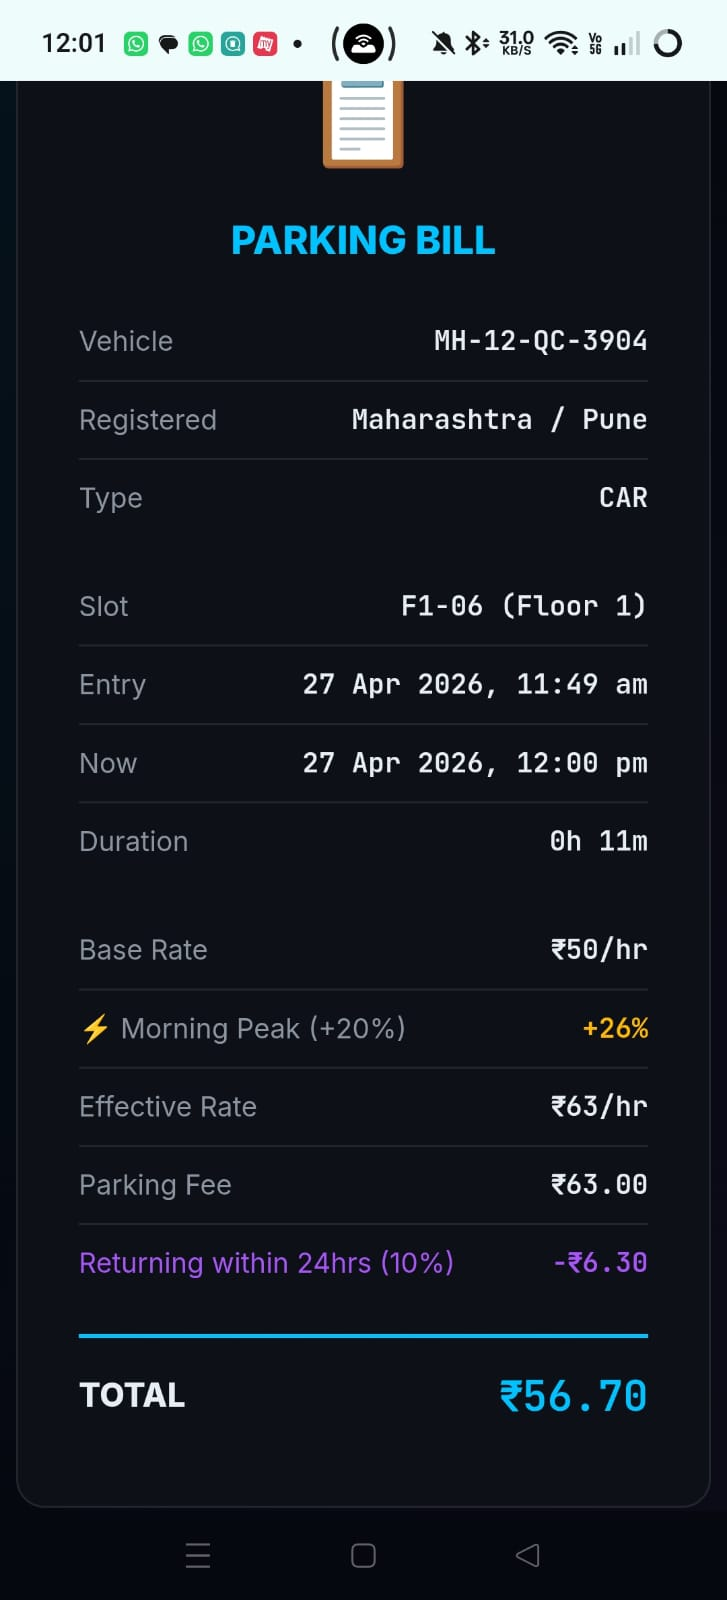
\includegraphics[width=0.85\textwidth]{../images/loyalty.jpeg}
    \caption{Returning Driver Loyalty Discount — Bill screen showing the discount tier, savings amount, and final discounted total for a returning vehicle.}
    \label{fig:loyalty}
\end{figure}

As shown in Figure~\ref{fig:loyalty}, the system automatically detects the returning vehicle and applies the appropriate discount tier. The bill clearly displays the original amount, the discount percentage, the savings, and the final amount the driver pays.

% ══════════════════════════════════════════════════════════
%  SECTION 4: RESULTS
% ══════════════════════════════════════════════════════════
\section{Results and Outcomes}

\subsection{Features Delivered}

\begin{table}[H]
\centering
\caption{Feature Delivery Status}
\begin{tabular}{|l|c|l|}
\hline
\textbf{Feature} & \textbf{Status} & \textbf{Notes} \\
\hline
findLastCompletedByVehicle() & \checkmark & SQL with ORDER BY + LIMIT \\
\hline
calculateLoyaltyDiscount() & \checkmark & 3-tier time gap analysis \\
\hline
applyDiscount() & \checkmark & Safe math with rounding \\
\hline
Lookup session integration & \checkmark & Bill preview shows discount \\
\hline
Checkout integration & \checkmark & Payment uses discounted total \\
\hline
Kiosk bill + payment screens & \checkmark & All 5 screens updated \\
\hline
Mobile bill + exit screens & \checkmark & Purple loyalty row \\
\hline
Receipt generation & \checkmark & Shows tier + saved amount \\
\hline
Try-catch safety wrapper & \checkmark & Non-fatal error handling \\
\hline
\end{tabular}
\end{table}

\subsection{Performance Metrics}

\begin{table}[H]
\centering
\caption{Enhancement Metrics}
\begin{tabular}{|l|l|}
\hline
\textbf{Metric} & \textbf{Value} \\
\hline
Discount tiers & 3 (10\%, 5\%, 2\%) \\
\hline
Surfaces updated & 7 (mobile bill, mobile exit, kiosk bill, cash, UPI, receipt, success) \\
\hline
Compounding & None (single highest tier only) \\
\hline
Applied to & Parking fee only (never fines) \\
\hline
Build status & BUILD SUCCESS (0 errors) \\
\hline
\end{tabular}
\end{table}

% ══════════════════════════════════════════════════════════
%  SECTION 5: CONCLUSION
% ══════════════════════════════════════════════════════════
\section{Conclusion}

The Returning Driver Loyalty Discount System transforms SnapPark's billing from a static fee calculator into a dynamic, customer-aware pricing engine. By leveraging historical session data and precise time gap analysis, the system rewards repeat customers with automatic discounts. The non-compounding tier design ensures simplicity and predictability, while the try-catch safety wrappers guarantee that discount calculation errors never block the checkout process. The feature is visible across all 7 billing surfaces, providing a consistent and professional user experience.

% ══════════════════════════════════════════════════════════
%  SECTION 6: LEARNING OUTCOMES
% ══════════════════════════════════════════════════════════
\section{Learning Outcomes}

\begin{itemize}
    \item \textbf{java.time API:} Used \texttt{Duration.between()}, \texttt{toHours()}, and \texttt{toDays()} for precise temporal calculations without external libraries.
    \item \textbf{SQL Query Design:} Wrote optimized queries with \texttt{ORDER BY ... DESC LIMIT 1} for efficient single-record retrieval.
    \item \textbf{Defensive Programming:} Wrapped all discount logic in try-catch blocks to ensure non-fatal failures in production.
    \item \textbf{Method Overloading:} Extended \texttt{generateReceipt()} with multiple signatures for backward compatibility.
    \item \textbf{Full-Stack Integration:} Propagated a single feature across DAO, Service, Controller, API, and UI layers consistently.
    \item \textbf{Non-Compounding Logic:} Implemented mutually exclusive tier selection using early-return pattern (if-return chains).
\end{itemize}

\end{document}
